\chapter[Uranium Enrichment Regression \newline Results and Discussion]{Uranium Enrichment Regression Results and Discussion}
% https://www.ncbi.nlm.nih.gov/pmc/articles/PMC5554294/

% great examples of various enriched U with a large range of detector resolutions https://www.lanl.gov/orgs/n/n1/docs/la_14206.pdf

% u232 origin, enrichment as function of u235 fraction https://www.pnnl.gov/main/publications/external/technical_reports/PNNL-12075.pdf

% Although mass spectrometry leads to very accurate analytical results, it has the drawbacks of high costs of the device and its operation involving a long process and destructive sample analysis [1], [2]. https://www.sciencedirect.com/science/article/pii/S1738573317308057#bib1

This chapter applies machine learning algorithms to measuring the $^{235}$U enrichment of infinitely thick samples of uranium in unknown shielding and scattering environments.

\section{Uranium Enrichment Measurement Background}

Verifying the enrichment of HEU through passive nondestructive analysis is important for nuclear safeguard applications and homeland security tasks. Passive nondestructive analysis, such as gamma-ray spectroscopy, is preferred to more accurate destructive methods due to its ability to operate quickly, preserve forensic evidence, and allow for remote measurements. The enriched uranium gamma-ray signatures visible in low-resolution detectors come from the decay of $^{238}$U, $^{235}$U, $^{232}$U, and the daughters of these isotopes. Figure \ref{fig:enriched_u_peaks_displayed} shows an example of a 27\% enriched uranium spectrum that displays $^{238}$U and $^{235}$U photopeaks. In low-resolution detectors, The primary photopeaks from $^{235}$U are at 144 keV, 163 keV, and 186 keV. The $^{238}$U daughter $^{234m}$Pa produces two main photopeaks at 766 keV and 1001 keV. $^{232}$U, only present in reprocessed uranium, produces a photopeak at 2.6 MeV from its $^{208}$Tl daughter.

\begin{figure}[H]
	\centering
	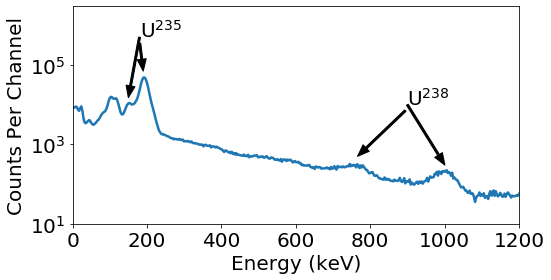
\includegraphics[width=0.8\linewidth]{images/enriched_u_peaks_displayed}
	\caption{27\% enriched uranium spectrum measured with a NaI detector.}.
	\label{fig:enriched_u_peaks_displayed}
\end{figure}

Traditionally, the enrichment meter method is used to measure uranium enrichment in NaI spectra \cite{Reilly1970}. This method exploits the proportionality between the activity of the 186 keV photon and the enrichment of $^{235}$U. The enrichment meter method works by finding calibration constants that relate counts in two ROIs,
%
\begin{align} \label{eq:enrichment_meter_principle}
E &= A  C_{ROI1} + B C_{ROI2} \nonumber \\
\text{where } C_{ROI1} &= \text{counts in ROI1 [\# counts]} \nonumber \\
C_{ROI2} &= \text{counts in ROI2 [\# counts]} \nonumber \\
A &= \text{calibration constant} \nonumber \\
B &= \text{calibration constant} \nonumber \\
\end{align}
%

to the enrichment of the measured material. These ROIs are placed around the 186 keV peak and in the background region to the right of the peak. Finding these constants requires measuring two different uranium enrichment standards in the same configuration (shielding, scattering environment, source-detector distance). Once these calibration constants are measured, they can only be used in the same configuration as the reference standards. It is possible to extend this method to other shielding configurations, but this introduces a risk of adding systematic errors. An automated version of this method called NaIGEM (NaI Gamma Enrichment Measurements) is included in the HM-5 instrument used by the IAEA \cite{MORTREAU2004}. Enrichment measurements of uranium without contaminants using low-resolution detectors can achieve 1\% precision for arbitrary enrichments while  contamination by minor uranium isotopes have a biasing effect of 5-10\% \cite{SPRINKLE1997}. Measurements of materials with unknown enrichment, shielding, and geometry are typically performed with high resolution HPGe detectors using the Multi-Group Analysis for Uranium (MGAU) software \cite{MGAU1994}.

% Measuring uranium enrichment with a NaI detector in an unknown configuration is difficult.


% Measuring the enrichment of uranium is made difficult by the fact that it's characteristic gamma-rays are easily shielded. This task is made more difficult for treaty verification by the restriction placed on inspectors. IAEA inspectors face two major restrictions: a limited amount of time to measure data from declared items and the requirement for an information barrier. This means that direct viewing and analysis of the gamma-ray spectrum - necessary for the enrichment meter method - is impossible. 


% "Generally, low resolution measurements of 'clean' uranium can be made to 1\% precision over nearly the entire range of uranium enrichment. Measurements in both Europe and the Former Soviet Union have observed bias effects of 5-10\% in low-resolution measurements caused by minor isotopes of uranium. This level of bias has been deemed unacceptable, causing some inspectors to resort to more expensive, time-consuming alternatives like mass spectrometry or liquid-nitrogen-cooler high-resolution detectors. As the international safeguards community attempts to inspect more facilities with less resources, these alternatives become highly undesirable. The minor isotopes come from the use of uranium recycled from reactors being used as feed in the enrichment plants. Daughters of $^{232}$U or $^{236}$U include the thorium decay chain which emits a 238.6-keV gamma ray from $^{212}$Pb. This gamma ray falls in the ROI used to estimate the Compton continuum under the 186-keV gamma ray. In addition, the multitude of high-energy gamma rays from the daughters of $^{232}$U change the shape of the Compton continuum that lies under the desired 186-keV peak. Just to make the entire issue more challenging, the level of this interference varies widely among the samples generally offered to the inspector, causing unpredictable, wide variations in the bias effects" \cite{SPRINKLE1997}

% Accuracies of +/- 10\% are expected for quick checks of high enriched material while accuracies of +/- 1\% are expected to verify mass spectroscopy measurments \cite{Kull1974}.

% Changes in background in the facility may affect performance. Studies done measuring uranium enrichment in marine environments have shown that background radiation is important and that existing methods  \cite{Hofstetter2008}.


\section{Problem Description and Training Dataset Overview}

To investigate how well a machine learning algorithm can learn to perform uranium enrichment measurements, machine learning architectures found in Chapter \ref{ChapterMachineLearningModelsExplored} were trained using a dataset of simulated enriched uranium spectra.

% u232 production reactions from uranium species https://www.pnnl.gov/main/publications/external/technical_reports/PNNL-12075.pdf

% FRAM application to U and Pu isotopics https://www.lanl.gov/orgs/n/n1/appnotes/LA-14018-M.pdf

\subsection{Training Dataset Details}

A coupled MCNP (Monte Carlo N-Particle Transport Code) and GADRAS-DRF code was used to simulate the spectrum from each uranium isotope uniformly distributed in a solid uranium sphere of radius 5.5 cm. The MCNP code was used to calculate the physics due to self attenuation in the uranium and GADRAS-DRF was used to model the gamma-ray spectrum from this source in a 2'' x 2'' NaI detector. The universe in the MCNP simulation, shown in Figure \ref{fig:mcnp_diagram}, was empty except for a 19 cm concrete block fixed at 180 cm from the origin, a 5.5 cm radius sphere of bare uranium fixed at the origin, and a bare 2'' x 2'' NaI cylinder located between them. The concrete block was added to incorporate backscatter radiation in the MCNP simulation. A total of 10$^{8}$ particles were simulated for each configuration.

\begin{figure}[H]
	\centering
    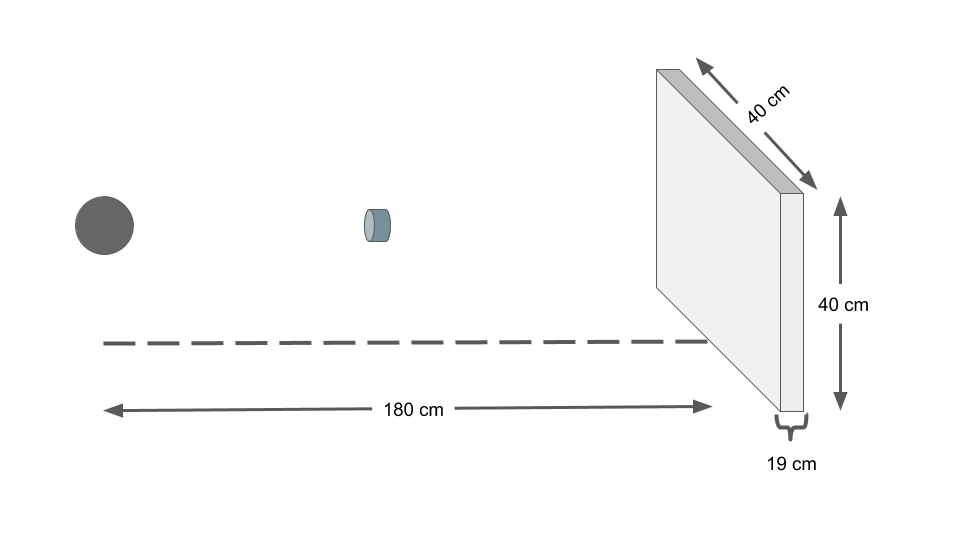
\includegraphics[trim=50 50 50 50,clip,width=0.99\linewidth]{images/mcnp_diagram.png}
	\caption{Diagram of MCNP simulation (not to scale).}
	\label{fig:mcnp_diagram}
\end{figure}

The software package RadSrc was used to generate specific gamma-ray intensities for the $^{235}$U, $^{238}$U, and $^{232}$U templates \cite{Hiller2007}. RadSrc, developed at Lawrence Livermore National Laboratory, uses the Bateman equations to calculate daughter in-growth and their respective specific gamma-ray intensities. Isotopes in enriched uranium reach secular equilibrium in about six months. To account for this, RadSrc was used to find specific gamma-ray intensities for 50 year old uranium isotopes and their ingrown daughters. The specific activities for each isotope are found in Table \ref{table:specific_activities_radsrc}.

\begin{table}[H]
\centering
\caption{Specific activities for 50 year old uranium isotopes and their ingrown daughters.}
\label{table:specific_activities_radsrc}
\begin{tabular}{ll}
% \cline{2-3}
% Isotope & photos/second/gram \\ \hline
% Isotope & $\frac{photos}{s g}$ \\ \hline
\hline
% Isotope & {\begin{tabular}[c]{@{}c@{}}Specific Gamma-ray\\ Intensities [$\gamma$/gram/second]\end{tabular}} \\ \hline
\textbf{Isotope} & \textbf{Specific Gamma-ray Activity [$\frac{\gamma}{g s}$]} \\ \hline
$^{232}$U & 1.20 x 10$^{12}$ \\ 
$^{235}$U & 2.07 x 10$^{5}$ \\
$^{238}$U & 3.80 x 10$^{3}$ \\ \hline
\end{tabular}
\end{table}


% (for example: burn-up conditions in the recycled material, enrichment process, )

$^{235}$U and $^{238}$U templates were combined based on the desired enrichment. To account for factors that change the $^{232}$U content, each sample that included $^{232}$U used a mass fraction uniformly chosen between 4 x 10$^{-9}$ and 2 x 10$^{-8}$ \cite{Peurrung2019}. To account for clean uranium, the probability that a spectrum was simulated with $^{232}$U was one half. Complete simulation parameters for the coupled MCNP and GADRAS-DRF code are shown in Table \ref{table:hyperparameter_dataset_full_parameters_enrichment}.

\begin{table}[H]
\centering
\caption{Range of parameters used for the uranium enrichment dataset.}
\label{table:hyperparameter_dataset_full_parameters_enrichment}
\begin{tabular}{lll}
\hline
\textbf{Simulation Parameter} & \textbf{Range} & \textbf{Sampling} \\ \hline
Source-Detector Distance [cm] & 25, 50, 100 & Uniform \\ % \hline
FWHM 662 keV [s] & 6.0, 6.5, 7.0, 7.5 & N/A \\ % \hline
Shielding (\% 200 keV Attenuated) & 0\%, 20\%, 40\%, 60\% & Uniform \\ % \hline
Integration Time [s] & 30 - 3600 & Log-Uniform \\ % \hline
Calibration Offset [channels] & -10 - 10 & Uniform \\ % \hline
Calibration Gain & 0.8 - 1.2 & Uniform \\ % \hline
$^{235}$U Enrichment [\%] & 0 - 100 & Uniform \\ % \hline
Background Counts per Second & 150 - 250 & Uniform \\ % \hline
Signal to Background Ratio & 0.1 - 4.0 & Uniform \\ \hline
\end{tabular}
\end{table}


\subsection{Training Outline}

Simple and complete model architectures discussed in Sections \ref{table:hyperparameter_opt_parameters_DNN} and \ref{table:hyperparameter_opt_parameters_CNN} were trained on a simulated dataset of 10$^{5}$ uranium spectra. Model architectures were modified to perform regression. Modifications include changing: the number of output nodes to one, their output function to a sigmoid, and their main cost function to mean squared error. Typically the sigmoid output function is used in the context of logistic regression. In our case the regression targets (percent $^{235}$U enrichment) exist on [0,1], allowing use of the sigmoid output function. Pretrained simple and complete DAE and CAE models from Section \ref{section_autoencoder_archetectures} were also fine-tuned using the simulated uranium dataset. Convolutional models were trained using 20 maximum epochs and a 5 epoch early stopping patience. Dense models were trained using 500 maximum epochs and a 50 epoch early stopping patience.

\section{Generalization Results - Simulated Data}

These sections describe how each trained model perform on simulated enriched uranium. To investigate the generalization performance, spectra are simulated with enrichments of 3\%, 25\%, 50\%, 75\%, and 93\% in different conditions. For each spectrum, the average output from five bagged trained models are recorded. To observe the output variance, 10 spectra are simulated for each enrichment value and their average output and variance are displayed. Default simulation parameters are shown in Table \ref{table:default_sim_params_uranium}. Changes to these defaults are indicated for each generalization experiment.

\begin{table}[H]
\centering
\caption{Default parameters used for all generalization datasets.}
\label{table:default_sim_params_uranium}
\begin{tabular}{ll}
\hline
\textbf{Simulation Parameter} &  \textbf{Value} \\ \hline
Source-Detector Distance [cm] & 50.0\\ 
FWHM 662 keV [s] & 7.0\\
Shielding (\% 200 keV Attenuated) & 0\% \\ 
Integration Time [s] & 600 \\ 
Calibration - Offset (channels) & 0 \\ 
Calibration - Gain & 1.0 \\ 
Signal to Background Ratio & 3.0 \\ 
Background Counts Per Second & 200 \\ \hline
\end{tabular}
\end{table}

\subsection{Generalization Results on Shielding}

To test each model's generalization performance with respect to shielding, enriched uranium spectra were simulated with various amounts of shielding. The effect of each shielding is shown in Figure \ref{fig:simulated_uranium_shielding}. The outputs from each model on these cases are shown in Figure \ref{fig:simuranium-shielding}. In general for each case, the complete networks outperform the simple networks. This indicates that the reduced capacity of the simple networks is insufficient to properly perform uranium enrichment measurements using the provided dataset. At 93\% enrichment each model underpredicted the enrichment.

The simple networks consistently overpredict the enrichment at and below 50\%. The simple models also underpredict the enrichment at values over 50\%. This reinforces the conclusion that the simple network has too little capacity to fit the data. Because the range of enrichments in the training data are uniformly distributed from 0 - 100\%, the naive method to minimize the cost function is to output values near 50\%. The simple networks, except for the simple DAE, consistently underpredicted the enrichment in the case with 1.42 mm lead shielding. The complete models were largely unaffected by the various amounts of shielding.


\begin{figure}[H]
	\centering
	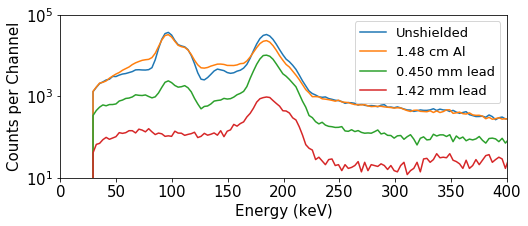
\includegraphics[width=0.8\linewidth]{images/simulated_uranium_shielding.png}
	\caption{Simulated 93\% enriched uranium spectra various amounts of shielding.}
	\label{fig:simulated_uranium_shielding}
\end{figure}

\begin{figure}[H]
     \centering
     \begin{subfigure}[b]{0.49\textwidth}
         \centering
         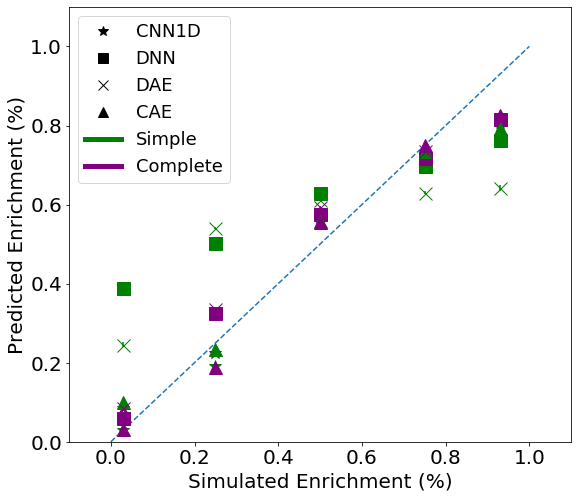
\includegraphics[width=\textwidth]{images/simuranium-noshield.png}
         \caption{Unshielded.}
         \label{fig:simuranium-noshield}
     \end{subfigure}
     \hfill
     \begin{subfigure}[b]{0.49\textwidth}
         \centering
         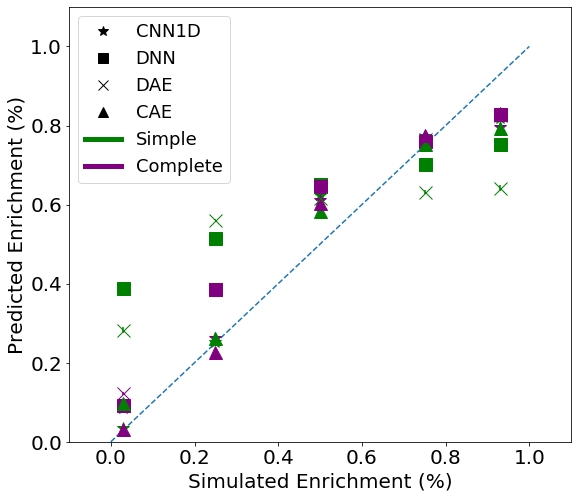
\includegraphics[width=\textwidth]{images/simuranium-lightal.png}
         \caption{1.48 cm aluminum.}
         \label{fig:simuranium-lightal}
     \end{subfigure}

     \begin{subfigure}[b]{0.49\textwidth}
         \centering
         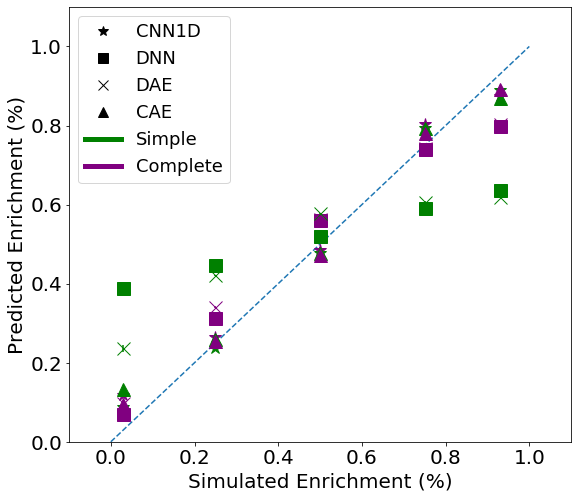
\includegraphics[width=\textwidth]{images/simuranium-mediumlead.png}
         \caption{0.450 mm lead.}
         \label{fig:simuranium-mediumlead}
     \end{subfigure}
     \hfill
     \begin{subfigure}[b]{0.49\textwidth}
         \centering
         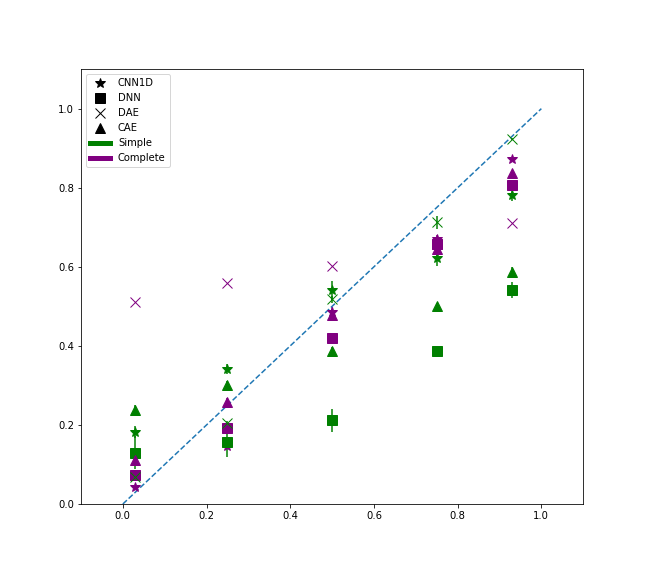
\includegraphics[width=\textwidth]{images/simuranium-heavylead.png}
         \caption{1.42 mm lead.}
         \label{fig:simuranium-heavylead}
     \end{subfigure}
        \caption{Shielding generalization performance in simulated enriched uranium spectra for the DNN, CNN with and without autoencoder pretraining. Simulated shielding amounts are indicated below each figure.} %Clockwise from the upper left, the shielding simulated are unshielded, 1.48 cm aluminum, 0.450 mm lead, and 1.42 mm lead.}
        \label{fig:simuranium-shielding}
\end{figure}




\subsection{Generalization Results on Changing Calibration} \label{section_uranium_sim_cal}

To test each model's generalization performance with respect to calibration, enriched uranium spectra were simulated with various relative gains. The outputs from each model on these cases are shown in Figure \ref{fig:simuranium-cal}. Model performance at relative gains of 0.9 and 1.1 are similar to the reference gain case, shown in Figure \ref{fig:simuranium-noshield}.

At the extreme relative gain shifts of 0.8 and 1.2 performance for the models changes. At a relative gain shift of 0.8, the dense models display a large variance in output values while the convolutional models do not. Convolutional models are effected less by the large change in gain because of their inherent shift invariance. At a relative gain shift of 0.8, the 186 keV peak from $^{235}$U is shifted to the 225 keV region as seen in Figure \ref{fig:simulated_uranium_calibration_93pct}. In this region there is little spectral information about enrichment. Because of this, this peak - which is the main source of enrichment information - may be ignored. Because the 186 keV peak is ignored the dense networks underpredict enrichment at a 0.8 relative gain shift. At a gain shift of 1.2 each model overpredicts enrichment for enrichments at and below 50\%. Because the 1.2 relative shift moves the 766 keV and 1001 keV $^{238}$U peaks into regions of little importance for the spectra without gain shift, seen in Figure \ref{fig:simulated_uranium_calibration_10pct}, these peaks are ignored and the enrichment is overpredicted.

% Also, because the shifted peak is wider, more nodes connected to this region would need to update to extract useful information. 


\begin{figure}[H]
     \centering
     \begin{subfigure}[b]{0.49\textwidth}
         \centering
         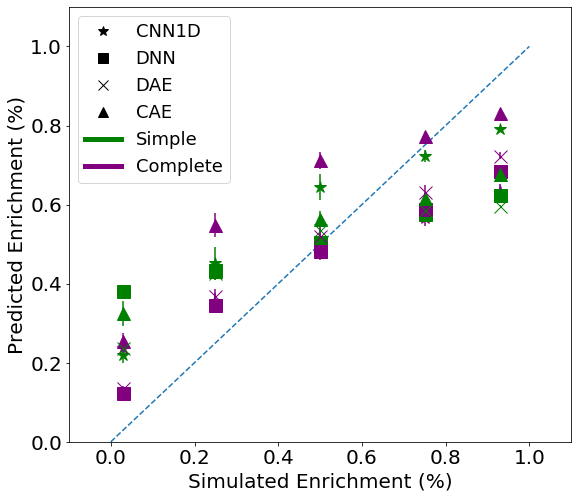
\includegraphics[width=\textwidth]{images/simuranium-cal08.png}
         \caption{0.8}
         \label{fig:simuranium-cal08}
     \end{subfigure}
     \hfill
     \begin{subfigure}[b]{0.49\textwidth}
         \centering
         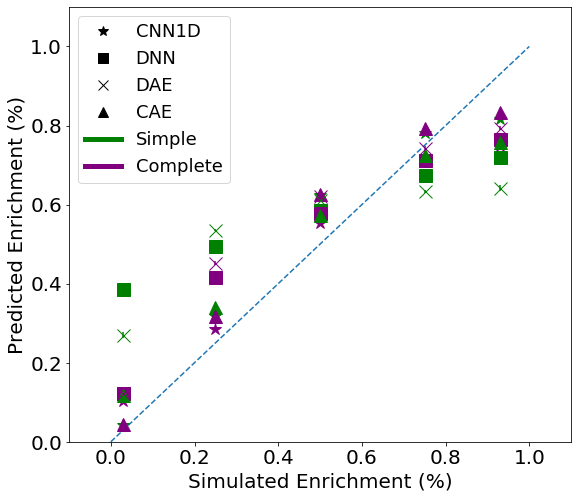
\includegraphics[width=\textwidth]{images/simuranium-cal09.png}
         \caption{0.9}
         \label{fig:simuranium-cal09}
     \end{subfigure}

     \begin{subfigure}[b]{0.49\textwidth}
         \centering
         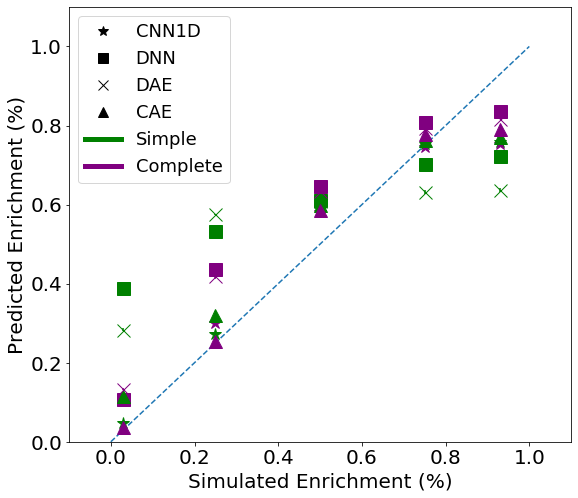
\includegraphics[width=\textwidth]{images/simuranium-cal11.png}
         \caption{1.1}
         \label{fig:simuranium-cal11}
     \end{subfigure}
     \hfill
     \begin{subfigure}[b]{0.49\textwidth}
         \centering
         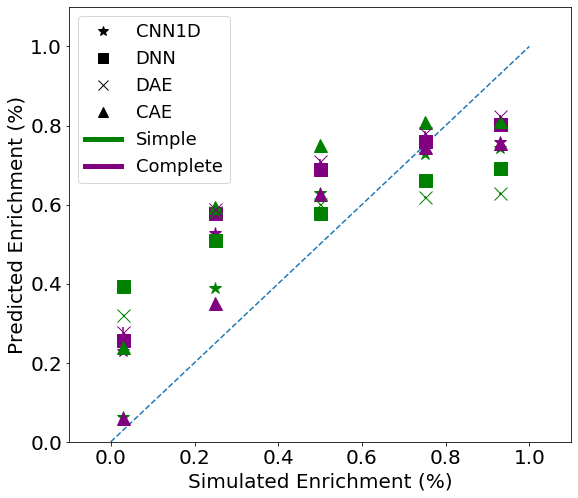
\includegraphics[width=\textwidth]{images/simuranium-cal12.png}
         \caption{1.2}
         \label{fig:simuranium-cal12}
     \end{subfigure}
        \caption{Calibration gain generalization performance in simulated spectra for the DNN, CNN with and without autoencoder pretraining. The magnitude of the applied relative gain shift are shown below each figure.}
        \label{fig:simuranium-cal}
\end{figure}





\begin{figure}[H]
	\centering
	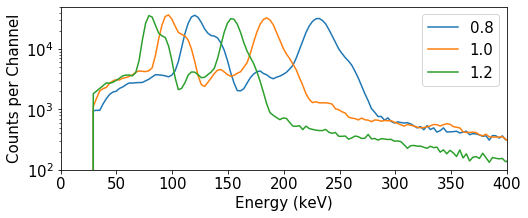
\includegraphics[width=0.8\linewidth]{images/simulated_uranium_calibration.png}
	\caption{Simulated 93\% enriched uranium spectra with three different relative gain settings. Energy calibration shown is based on the 1.0 relative gain setting.}
	\label{fig:simulated_uranium_calibration_93pct}
\end{figure}

\begin{figure}[H]
	\centering
	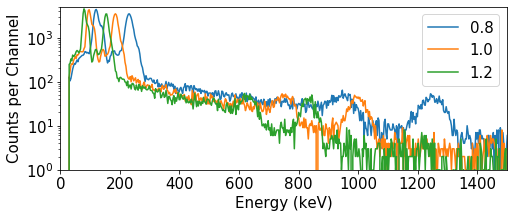
\includegraphics[width=0.8\linewidth]{images/simulated_uranium_calibration_1500kev.png}
	\caption{Simulated 10\% enriched uranium spectra with three different relative gain settings. Energy calibration shown is based on the 1.0 relative gain setting.}
	\label{fig:simulated_uranium_calibration_10pct}
\end{figure}

\section{Results - Measured Spectra}

Spectra of various uranium enrichments from a variety of NaI detectors were collected and the each model's response was recorded. Measured spectra include a 13 kg 93\% enriched uranium metal sphere \cite{Rothe1997} and U$_{3}$O$_{8}$ measured at lower enrichments. The U$_{3}$O$_{8}$ spectra were measured with as part of an IAEA measurement exercises which did not measure energies above 1.3 MeV. This should have little effect on the regression because if models learned to ignore this region which contains no enrichment information. In addition to this, the calibration of the detectors were not the same. For testing purposes, each spectrum was manually recalibrated using gain and offset correction to recalibrate the 186 keV and 1001 keV photopeaks. These recalibrated spectra are shown in Figure \ref{fig:measured_uranium_plots}. Shielding, source-detector distance, radiation background, and scattering environments are unknown for the U$_{3}$O$_{8}$ spectra.

\begin{table}[H]
\centering
\caption{Uranium sample description.}
\label{table:uranium_sample_description}
\begin{tabular}{cccc}
\hline
Enrichment & $^{235}$U Mass (g) & Material & Live Time (s)   \\ \hline
93.1\% & 13,000 & U Metal & 300 \\
91.4\% & 903 & U$_{3}$O$_{8}$ &  226\\
27.1\%  & 264 & U$_{3}$O$_{8}$ & 344 \\ 
0.7\% & - & U$_{3}$O$_{8}$ & 97.4 \\ \hline
\end{tabular}
\end{table}

\begin{figure}[H]
	\centering
	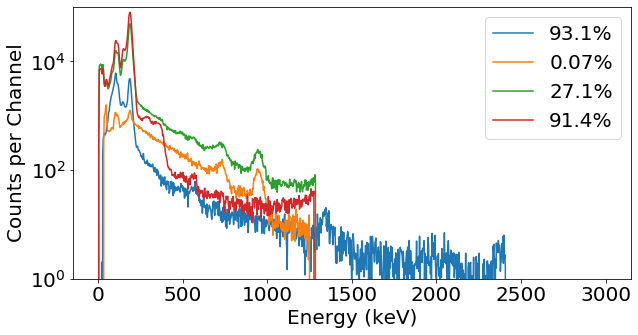
\includegraphics[width=0.8\linewidth]{images/measured_uranium_plots.png}
	\caption{Enriched uranium spectra recalibrated to the 186 keV and 1001 keV photopeaks.}
	\label{fig:measured_uranium_plots}
\end{figure}

Figure \ref{fig:measured_uranium} shows the mean and variance of each model and each measured spectrum. Similar to the simulated spectra, the simple architectures underpredicted enrichments over 50\% and overpredicted enrichments under 50\%. The simple DAE had a visible output variance at lower enrichments while the rest of the networks did not have observable variance in their outputs. The complete architectures were more accurate than the simple architectures above 20\% enrichment. At 27.1\% enrichment, each convolutional model overpredicted the enrichment while the dense models predicted closer to the true value. % This is due to the $^{235}$U features being the wrong size for the convolutional filters.



\begin{figure}[H]
	\centering
	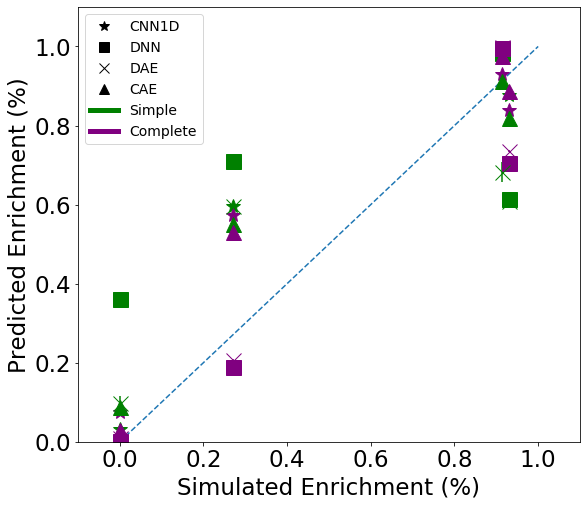
\includegraphics[width=0.8\linewidth]{images/measured_uranium.png}
	\caption{Results from measured uranium of different enrichments.}
	\label{fig:measured_uranium}
\end{figure}

To investigate how changing calibration effects each algorithm, the recalibrated spectra were additionally recalibrated with the same gain settings explored in Section \ref{section_uranium_sim_cal}. 

Similar to the simulated results, gain changes of 0.9 and 1.1 do not significantly impact enrichment quantification for the complete networks. An exception to this is the complete dense models underpredict enrichment in the 93\% enriched, 1.1 gain setting spectrum. At a gain of 0.8, networks generally overpredicted the enrichment of lower enrichment samples. This effect was observed to a smaller magnitude in simulated results.

\begin{figure}[H]
     \centering
     \begin{subfigure}[b]{0.49\textwidth}
         \centering
         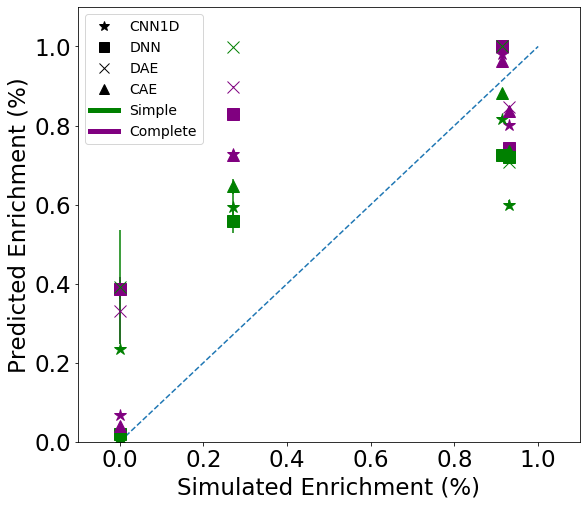
\includegraphics[width=\textwidth]{images/measured_uranium_08.png}
         \caption{0.8}
         \label{fig:measured_uranium_08}
     \end{subfigure}
     \hfill
     \begin{subfigure}[b]{0.49\textwidth}
         \centering
         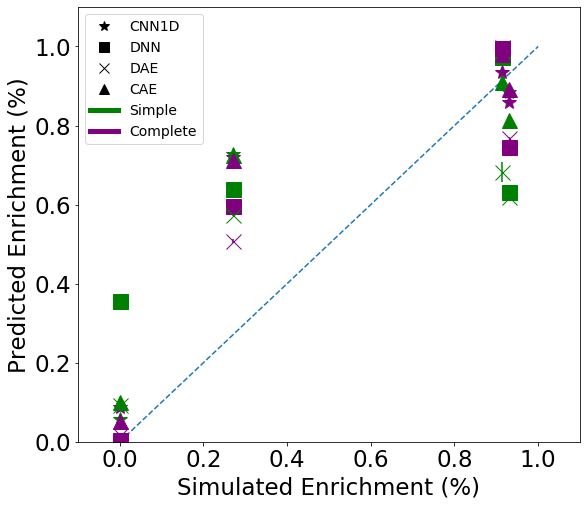
\includegraphics[width=\textwidth]{images/measured_uranium_09.png}
         \caption{0.9}
         \label{fig:measured_uranium_09}
     \end{subfigure}

     \begin{subfigure}[b]{0.49\textwidth}
         \centering
         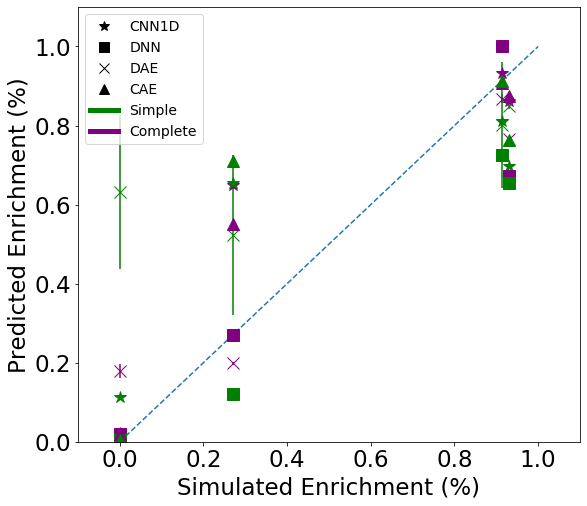
\includegraphics[width=\textwidth]{images/measured_uranium_11.png}
         \caption{1.1}
         \label{fig:measured_uranium_11}
     \end{subfigure}
     \hfill
     \begin{subfigure}[b]{0.49\textwidth}
         \centering
         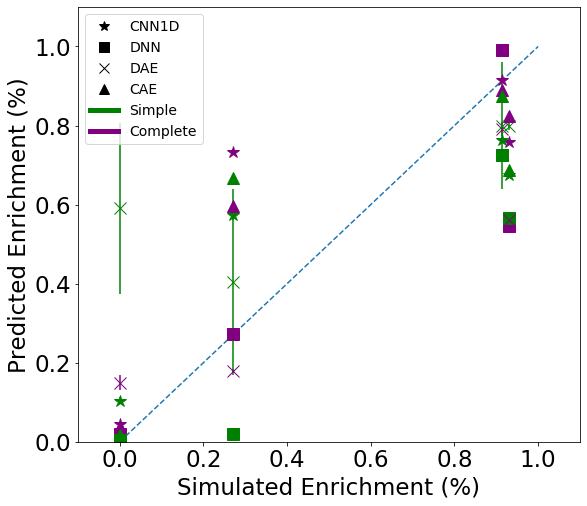
\includegraphics[width=\textwidth]{images/measured_uranium_12.png}
         \caption{1.2}
         \label{fig:measured_uranium_12}
     \end{subfigure}
        \caption{Calibration gain generalization performance in recalibrated measured spectra for the DNN, CNN with and without autoencoder pretraining. The magnitude of the applied relative gain shift are shown below each figure.}
        \label{fig:realuranium-cal}
\end{figure}



\section{Discussion and Conclusion}

This chapter shows that the complete architectures outperform the simple architectures on uranium enrichment regression tasks. The results also show that the complete architectures are well suited to extend to other problems in gamma-ray spectroscopy. The chapter also demonstrates that autoencoders trained to reconstruct unrelated spectra are useful as pretraining for other spectroscopic tasks. The DAE performed particularly well on simulated and measured data in various conditions. Dense models show promise in uranium enrichment regression. This may be because aspects of the feature extraction processes in the convolution architectures are tuned to general isotope identification. Uranium enrichment regression may require convolution window sizes smaller than those in the simple or complete dataset (8 and 16 channels) to better extract narrow photopeaks below 200 keV. 

While the current implementation can roughly differentiate between low and high enriched uranium, the training set needs to be expanded to achieve useful accuracy for international safeguards measurements or homeland security surveys. Additional scattering scenarios simulating cargo containers and small uranium samples that cannot be assumed to be infinitely thick at 186 keV could be added. The $^{232}$U content could also be modeled more accurately \cite{Peurrung2019}.

% Additional examples need to $^{241}$Am, $^{239}$Pu, and $^{237}$Np from recycled uranium. 

% Bremsstrahlung from the $^{234m}$Tl, a $^{238}$U daughter, could be added to the simulations to make low-enrichment measurements more accurate.





